\documentclass[12pt, a4paper]{article}

%<*preamble>
% Math symbols
\usepackage{amsmath, amsthm, amsfonts, amssymb}
\usepackage{accents}
\usepackage{esvect}
\usepackage{mathrsfs}
\usepackage{mathtools}
\mathtoolsset{showonlyrefs}
\usepackage{cmll}
\usepackage{stmaryrd}
\usepackage{physics}
\usepackage[normalem]{ulem}
\usepackage{ebproof}
\usepackage{extarrows}

% Page layout
\usepackage{geometry, a4wide, parskip, fancyhdr}

% Font, encoding, russian support
\usepackage[russian]{babel}
\usepackage[sb]{libertine}
\usepackage{xltxtra}

% Listings
\usepackage{listings}
\lstset{basicstyle=\ttfamily,breaklines=true}
\setmonofont{Inconsolata}

% Miscellaneous
\usepackage{array}
\usepackage{calc}
\usepackage{caption}
\usepackage{subcaption}
\captionsetup{justification=centering,margin=2cm}
\usepackage{catchfilebetweentags}
\usepackage{enumitem}
\usepackage{etoolbox}
\usepackage{float}
\usepackage{lastpage}
\usepackage{minted}
\usepackage{svg}
\usepackage{wrapfig}
\usepackage{xcolor}
\usepackage[makeroom]{cancel}

\newcolumntype{L}{>{$}l<{$}}
    \newcolumntype{C}{>{$}c<{$}}
\newcolumntype{R}{>{$}r<{$}}

% Footnotes
\usepackage[hang]{footmisc}
\setlength{\footnotemargin}{2mm}
\makeatletter
\def\blfootnote{\gdef\@thefnmark{}\@footnotetext}
\makeatother

% References
\usepackage{hyperref}
\hypersetup{
    colorlinks,
    linkcolor={blue!80!black},
    citecolor={blue!80!black},
    urlcolor={blue!80!black},
}

% tikz
\usepackage{tikz}
\usepackage{tikz-cd}
\usetikzlibrary{arrows.meta}
\usetikzlibrary{decorations.pathmorphing}
\usetikzlibrary{calc}
\usetikzlibrary{patterns}
\usepackage{pgfplots}
\pgfplotsset{width=10cm,compat=1.9}
\newcommand\irregularcircle[2]{% radius, irregularity
    \pgfextra {\pgfmathsetmacro\len{(#1)+rand*(#2)}}
    +(0:\len pt)
    \foreach \a in {10,20,...,350}{
            \pgfextra {\pgfmathsetmacro\len{(#1)+rand*(#2)}}
            -- +(\a:\len pt)
        } -- cycle
}

\providetoggle{useproofs}
\settoggle{useproofs}{false}

\pagestyle{fancy}
\lfoot{M3137y2019}
\cfoot{}
\rhead{стр. \thepage\ из \pageref*{LastPage}}

\newcommand{\R}{\mathbb{R}}
\newcommand{\Q}{\mathbb{Q}}
\newcommand{\Z}{\mathbb{Z}}
\newcommand{\B}{\mathbb{B}}
\newcommand{\N}{\mathbb{N}}
\renewcommand{\Re}{\mathfrak{R}}
\renewcommand{\Im}{\mathfrak{I}}

\newcommand{\const}{\text{const}}
\newcommand{\cond}{\text{cond}}

\newcommand{\teormin}{\textcolor{red}{!}\ }

\DeclareMathOperator*{\xor}{\oplus}
\DeclareMathOperator*{\equ}{\sim}
\DeclareMathOperator{\sign}{\text{sign}}
\DeclareMathOperator{\Sym}{\text{Sym}}
\DeclareMathOperator{\Asym}{\text{Asym}}

\DeclarePairedDelimiter{\ceil}{\lceil}{\rceil}

% godel
\newbox\gnBoxA
\newdimen\gnCornerHgt
\setbox\gnBoxA=\hbox{$\ulcorner$}
\global\gnCornerHgt=\ht\gnBoxA
\newdimen\gnArgHgt
\def\godel #1{%
    \setbox\gnBoxA=\hbox{$#1$}%
    \gnArgHgt=\ht\gnBoxA%
    \ifnum     \gnArgHgt<\gnCornerHgt \gnArgHgt=0pt%
    \else \advance \gnArgHgt by -\gnCornerHgt%
    \fi \raise\gnArgHgt\hbox{$\ulcorner$} \box\gnBoxA %
    \raise\gnArgHgt\hbox{$\urcorner$}}

% \theoremstyle{plain}

\theoremstyle{definition}
\newtheorem{theorem}{Теорема}
\newtheorem*{definition}{Определение}
\newtheorem{axiom}{Аксиома}
\newtheorem*{axiom*}{Аксиома}
\newtheorem{lemma}{Лемма}

\theoremstyle{remark}
\newtheorem*{remark}{Примечание}
\newtheorem*{exercise}{Упражнение}
\newtheorem{corollary}{Следствие}[theorem]
\newtheorem*{statement}{Утверждение}
\newtheorem*{corollary*}{Следствие}
\newtheorem*{example}{Пример}
\newtheorem{observation}{Наблюдение}
\newtheorem*{prop}{Свойства}
\newtheorem*{obozn}{Обозначение}

% subtheorem
\makeatletter
\newenvironment{subtheorem}[1]{%
    \def\subtheoremcounter{#1}%
    \refstepcounter{#1}%
    \protected@edef\theparentnumber{\csname the#1\endcsname}%
    \setcounter{parentnumber}{\value{#1}}%
    \setcounter{#1}{0}%
    \expandafter\def\csname the#1\endcsname{\theparentnumber.\Alph{#1}}%
    \ignorespaces
}{%
    \setcounter{\subtheoremcounter}{\value{parentnumber}}%
    \ignorespacesafterend
}
\makeatother
\newcounter{parentnumber}

\newtheorem{manualtheoreminner}{Теорема}
\newenvironment{manualtheorem}[1]{%
    \renewcommand\themanualtheoreminner{#1}%
    \manualtheoreminner
}{\endmanualtheoreminner}

\newcommand{\dbltilde}[1]{\accentset{\approx}{#1}}
\newcommand{\intt}{\int\!}

% magical thing that fixes paragraphs
\makeatletter
\patchcmd{\CatchFBT@Fin@l}{\endlinechar\m@ne}{}
{}{\typeout{Unsuccessful patch!}}
\makeatother

\newcommand{\get}[2]{
    \ExecuteMetaData[#1]{#2}
}

\newcommand{\getproof}[2]{
    \iftoggle{useproofs}{\ExecuteMetaData[#1]{#2proof}}{}
}

\newcommand{\getwithproof}[2]{
    \get{#1}{#2}
    \getproof{#1}{#2}
}

\newcommand{\import}[3]{
    \subsection{#1}
    \getwithproof{#2}{#3}
}

\newcommand{\given}[1]{
    Дано выше. (\ref{#1}, стр. \pageref{#1})
}

\renewcommand{\ker}{\text{Ker }}
\newcommand{\im}{\text{Im }}
\renewcommand{\grad}{\text{grad}}
\newcommand{\rg}{\text{rg}}
\newcommand{\defeq}{\stackrel{\text{def}}{=}}
\newcommand{\defeqfor}[1]{\stackrel{\text{def } #1}{=}}
\newcommand{\itemfix}{\leavevmode\makeatletter\makeatother}
\newcommand{\?}{\textcolor{red}{???}}
\renewcommand{\emptyset}{\varnothing}
\newcommand{\longarrow}[1]{\xRightarrow[#1]{\qquad}}
\DeclareMathOperator*{\esup}{\text{ess sup}}
\newcommand\smallO{
    \mathchoice
    {{\scriptstyle\mathcal{O}}}% \displaystyle
    {{\scriptstyle\mathcal{O}}}% \textstyle
    {{\scriptscriptstyle\mathcal{O}}}% \scriptstyle
    {\scalebox{.6}{$\scriptscriptstyle\mathcal{O}$}}%\scriptscriptstyle
}
\renewcommand{\div}{\text{div}\ }
\newcommand{\rot}{\text{rot}\ }
\newcommand{\cov}{\text{cov}}

\makeatletter
\newcommand{\oplabel}[1]{\refstepcounter{equation}(\theequation\ltx@label{#1})}
\makeatother

\newcommand{\symref}[2]{\stackrel{\oplabel{#1}}{#2}}
\newcommand{\symrefeq}[1]{\symref{#1}{=}}

% xrightrightarrows
\makeatletter
\newcommand*{\relrelbarsep}{.386ex}
\newcommand*{\relrelbar}{%
    \mathrel{%
        \mathpalette\@relrelbar\relrelbarsep
    }%
}
\newcommand*{\@relrelbar}[2]{%
    \raise#2\hbox to 0pt{$\m@th#1\relbar$\hss}%
    \lower#2\hbox{$\m@th#1\relbar$}%
}
\providecommand*{\rightrightarrowsfill@}{%
    \arrowfill@\relrelbar\relrelbar\rightrightarrows
}
\providecommand*{\leftleftarrowsfill@}{%
    \arrowfill@\leftleftarrows\relrelbar\relrelbar
}
\providecommand*{\xrightrightarrows}[2][]{%
    \ext@arrow 0359\rightrightarrowsfill@{#1}{#2}%
}
\providecommand*{\xleftleftarrows}[2][]{%
    \ext@arrow 3095\leftleftarrowsfill@{#1}{#2}%
}

\allowdisplaybreaks

\newcommand{\unfinished}{\textcolor{red}{Не дописано}}

% Reproducible pdf builds 
\special{pdf:trailerid [
<00112233445566778899aabbccddeeff>
<00112233445566778899aabbccddeeff>
]}
%</preamble>


\lhead{Математический анализ}
\cfoot{}
\rfoot{21.9.2020}

\begin{document}

% \begin{example}
%     Загадка. $f(x, y) = x^2 + Axy^2 + y^4$.

%     $(a, 0)$ --- подозрительная точка, $d^2f = 2dx^2 \ge 0$

%     $f(x_0 + h) \stackrel{\text{Тейлор}}{=} f(x_0) + \underbrace{df(x_0, h)}_{0} + \frac{1}{2}d^2 f(x_0, h) + \frac{1}{3!} d^3f(x_0, h) + \frac{1}{4!}d^4f(x_0, h)$
% \end{example}

В первом семестре была задача нахождения максимального по площади вписанного $n$-угольника.
Мы выяснили, что если максимум существует, то он достигается правильным $n$-угольником (\textit{суждение про сдвиг точки}). Кроме того, мы доказали, что максимум существует, сделаем это снова, но другим методом.

\begin{proof}
    Пусть внутренние углы многоугольника $\varphi_1\ldots \varphi_n$, тогда
    \begin{align*}
        S & = \frac{1}{2} r^2(\sin \varphi_1 + \ldots + \sin \varphi_n)                                                 \\
          & = \frac{1}{2} r^2(\sin \varphi_1 + \ldots + \sin \varphi_{n-1} - \sin (\varphi_1 - \ldots - \varphi_{n-1}))
    \end{align*}

    Очевидно $\forall i \ \ 0<\varphi_1<\pi \quad \pi < \varphi_1+\ldots+\varphi_{n-1} < 2\pi$.

    Найдём максимум путём дифференцирования. Это требует существования максимума внутри области определения. Если все неравенства сделать нестрогими, то область определения становится замкнутой, очевидно ограниченной $\Rightarrow \exists \max$ по теореме Вейерштрасса. Кроме того, максимум не лежит на границе области определения из очевидных геометрических соображений.

    $$\frac{\partial S}{\partial \varphi_i} = 0 \Leftrightarrow \cos \varphi_i = \cos(\varphi_1+\ldots+\varphi_{n-1})$$
    \begin{align*}
        \cos \varphi_i - \cos(\varphi_1+\ldots+\varphi_{n-1})   & = 0              \\
        2\sin \frac{n\varphi}{2} \sin \frac{\pi - 2n\varphi}{2} & = 0              \\
        \varphi                                                 & = \frac{2\pi}{n} \\
    \end{align*}
\end{proof}

\section*{Диффеоморфизмы}

\begin{definition}
    \textbf{Область} --- открытое связное множество.
\end{definition}

\begin{definition}
    $F : \underbrace{O}_{\text{область}}\subset \R^m\to \R^m$ --- \textbf{диффеоморфизм}, если:
    \begin{itemize}
        \item $F$ обратимо
        \item $F$ дифференцируемо
        \item $F^{-1}$ дифференцируемо
    \end{itemize}
\end{definition}
\begin{remark}
    $Id = F\circ F^{-1} = F^{-1}\circ F$

    $E = F' (F^{-1})' \Rightarrow \forall x \ \ \det F'(x) \not=0$
\end{remark}

\begin{lemma}[о почти локальной иньективности]\itemfix
    \begin{itemize}
        \item $F : O\subset\R^m\to\R^m$
        \item $F$ дифф. в $x_0\in O$
        \item $\det F'(x_0)\not=0$
    \end{itemize}
    Тогда $\exists c>0, \delta>0 \ \ \forall h < \delta \ \ |F(x_0+h)-F(x_0)| > C|h|$
\end{lemma}
\begin{proof}
    Если $F$ --- линейное отображение:
    $$|F(x_0+h) - F(x_0)| = |F(h)| = |F'(x_0)h| \ge ||F'(x_0)||\cdot |h| \ge \frac{1}{||(F'(x_0))^{-1}||}|h|$$
    $$|F(x_0+h) - F(x_0)| = |F'(x_0)h + \alpha(h)|h|| \ge c|h| - \frac{c}{2}|h| \ge \frac{c}{2}|h|$$
\end{proof}

\begin{theorem}[о сохранении области]\itemfix
    \begin{itemize}
        \item $F : O\subset\R^m \to\R^m$
        \item $F$ дифф.
        \item $\forall x\in O \ \ \det F'(x)\not=0$
    \end{itemize}
    Тогда $F(O)$ --- открыто.
\end{theorem}

\begin{remark}
    $O$ --- связно, $F$ --- непр. $\Rightarrow F(O)$ связно.
\end{remark}

\begin{proof}
    $x_0 \in O \Rightarrow F(x_0)\in F(O)$ --- внутренняя? в $F(O)$

    По лемме $\exists c, \delta : \forall h \in \overline{B(0, \delta)} \ \ |F(x_0+h) - F(x_0)| > C|h|$

    В частности $F(x_0 + h)\not=F(x_0)$ при $|h| = \delta$

    $$r := \frac{1}{2}\rho(y_0, F(S(x_0, \delta))$$
    $$\rho(A, B) \defeq \inf_{a\in A, b\in B} \rho(a, b)$$
    Т.к. $S$ --- компакт, $\exists \min$.

    Если $y\in B(y_0, r)$, то $\rho(y, F(S(x_0, \delta))) > r$:
    \begin{figure}[h]
        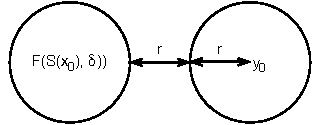
\includegraphics{images/осохраненииобласти.pdf}
        \centering
    \end{figure}

    \pagebreak

    Проверим, что $B(y_0, r) \subset F(O)$, т.е. $\forall y\in B(y_0, r) \ \ \exists x\in B(x_0, \delta) \ \ F(x) = y$

    Рассмотрим функцию $g(x) = |F(x) - y|^2$ при $x\in \overline{B(x_0, \delta)}$.

    Мы хотим показать, что $\exists x : g(x) = 0$. Найдем $\min g$.
    $$g(x_0) = |F(x_0) - y|^2 = |y_0 - y|^2 < r^2$$
    При $x\in S(x_0, \delta) : g(x)>r^2 \Rightarrow \min g$ не лежит на границе шара $\Rightarrow$ он лежит внутри шара.

    $$g(x) = (F_1(x) - y_1)^2 + \ldots + (F_m(x) - y_m)^2$$
    $$\forall i \quad \frac{\partial g}{\partial x_i} = 0$$
    $$2(F_1(x) - y)F'_{1x_i}(x) + \ldots + 2(F_m(x) - y)F'_{mx_i}(x) = 0$$
    $$F'_x 2(F(x) - y) = 0$$
    $$\forall x \ \ \det F'\not=0 \Rightarrow F(x) - y = 0$$
\end{proof}

\begin{corollary}\itemfix
    \begin{itemize}
        \item $F : O\subset\R^m \to\R^l$
        \item $F \in C^1(O)$
        \item $l < m$
        \item $\rg F'(x) = l \ \ \forall x\in O$
    \end{itemize}
    Тогда $F(O)$ открыто.
\end{corollary}
\begin{proof}
    Зафискируем точку $x_0$. Пусть ранг реализуется на столбцах $1\ldots l$, т.е. определитель матрицы из столбцов $1\ldots l \not=0$, т.е.:
    $$\det\underbrace{\left(\frac{\partial F_i}{\partial x_j}\right)_{i, j = 1\ldots l}(x_0)}_{A(x_0)} \not = 0$$
    И для близких точек тоже $\not=0$
    $$\tilde F : O \to\R^m \quad \tilde F(x) = \begin{pmatrix}
            F_1(x)  \\
            F_2(x)  \\
            \vdots  \\
            F_l(x)  \\
            x_{l+1} \\
            \vdots  \\
            x_m
        \end{pmatrix}$$
    $$\tilde F'(x) = \left[\begin{array}{cc}
                \multicolumn{2}{c}{F'(x)}        \\
                \hline
                \multicolumn{1}{c|}{0} & E_{m-l} \\
            \end{array}\right]$$
    $$\det \tilde F'(x) = \det A(x) \det E_{m-l} \not= 0 \ \ \text{ в окрестности } x_0$$

    Тогда $\tilde F\Big|_{U(x_0)}$ удовлетворяет теореме $\Rightarrow \tilde F(U(x_0))$ --- открытое множество в $\R^m$

    $F(U(x_0)) = \tilde F(U(x_0)) \cap \R^l$
\end{proof}

\begin{theorem}[о гладкости обратного отображения]\itemfix
    \begin{itemize}
        \item $T \in C^r(O, \R^m)$
        \item $O\subset\R^m$
        \item $r = 1, 2, \ldots +\infty$
        \item $T$ обратимо
        \item $\det T'(x) \not=0 \ \ \forall x\in O$
    \end{itemize}
    Тогда $T^{-1} \in C^r(0, \R^m)$ и $(T^{-1})'_{y_0} = (T'(x_0))^{-1}$, где $y_0 = T(x_0)$
\end{theorem}
\begin{proof}
    Докажем по индукции по $r$.

    \textbf{База}: $r = 1$

    $S := T^{-1}$ --- непрерывно по теореме о сохранении области. Почему?

    $f : X \to Y$ непр. $\Leftrightarrow \forall B$ --- откр. $\subset Y$ $f^{-1}(B)$ --- открыто.

    $T'(x_0) = A$ --- невырожденный оператор.

    По лемме о локальной иньективности
    $$\exists c, \delta : \forall x\in B(x_0, \delta) \ \ |T(x) - T(x_0)| > C|x-x_0| \quad (*)$$

    По определению дифференцируемости $T(x) - T(x_0) = A(x-x_0) + \omega(x)|x-x_0|$

    $$T(x) = y \quad T(x_0) = y_0 \quad x = S(y) \quad x_0 = S(x_0)$$

    В терминах $y$ и $S$:
    $$S(y) - S(y_0) = A^{-1}(y-y_0) - \underbrace{A^{-1}\omega(S(y))|S(y)-S(y_0)|}_{\xrightarrow[y\to0]{?}0 \text{ быстрее, чем } |y-y_0|}$$
    Если действительно $\to0$, то $S$ дифференцируемо по определению.

    Пусть $y$ близко к $y_0$, тогда $|x-x_0| = |S(y) - S(y_0)| < \delta$
    \begin{align*}
        |A^{-1}w(S(y))|S(y) - S(y_0)|| & = |S(y) - S(y_0)|\cdot|A^{-1}w(S(y))|                                    \\
                                       & \le |x-x_0| \cdot ||A^{-1}|| \cdot |w(S(y))|                             \\
                                       & \stackrel{(*)}{\le} \frac{1}{C}|y - y_0|\cdot ||A^{-1}|| \cdot |w(S(y))|
    \end{align*}

    Мы доказали, что $S$ дифференцируемо, теперь необходимо доказать, что $S'$ непрерывно.

    $$S'(y_0) = A^{-1}$$
    ``Алгоритм'' получения обратного оператора:
    $$y \mapsto T^{-1}(y) = x\mapsto T'(x) = A \mapsto A^{-1}$$

    Здесь все шаги непрерывны, поэтому $S'$ непрерывно.

    \textbf{Переход}

    $$T \in C^{r+1} \quad T' : O\to\mathcal L(\R^n, \R^n) \quad T'\in C^{r} \quad ? S\in C^{r+1}$$
    $$y \stackrel{\in C^r \text{ по инд.}}{\mapsto} S(y) \stackrel{\in C^r}{\mapsto} T'(x) \stackrel{\in C^\infty}{\mapsto} (S^{-1})'$$
\end{proof}

\begin{theorem}[о локальной обратимости]\itemfix
    \begin{itemize}
        \item $T\in C^r(O, \R^m)$
        \item $x_0\in O$
        \item $\det T'(x_0)\not=0$
    \end{itemize}
    Тогда $\exists U(x_0) : T\Big|_{U}$ --- диффеоморфизм, т.е. $\exists T^{-1}$

    Формулировака в терминах системы уравнений:
    $$\begin{cases}
            f_1(x_1\ldots x_m) = y_1 \\
            f_2(x_1\ldots x_m) = y_2 \\
            \vdots                   \\
            f_m(x_1\ldots x_m) = y_m \\
        \end{cases}$$
    Пусть $(x^0, y^0)$ --- решение этой системы, $F = (f_1\ldots f_m)$

    $\det F'(x^0) \not=0$. Тогда $\exists U(y^0) : \forall y\in U(y^0)$ система имеет решение, $C^r$ гладко зависящее от $y$.
\end{theorem}

\begin{theorem}[о неявном отображении]\itemfix
    \begin{itemize}
        \item $F : O\subset\R^{m+n} \to\R^n$
        \item $F\in\C^r$
        \item $(a, b)\in O$
        \item $F(a, b) = 0$
        \item $\det \left(\frac{\partial F_i}{\partial y_j}(a, b)\right)_{i, j = 1\ldots n} \not=0$
    \end{itemize}

    Будем считать $(x, y)\in\R^{m+n}$, где $x\in\R^m, y\in\R^n$ и первые $m$ координат $(x, y)$ --- координаты $x$, остальные --- координаты $y$.

    Тогда $\exists P(a)\subset\R^m, Q(b)\subset\R^n$ --- окрестности, $\exists \varphi : P(a) \to Q(b) \in C^r$, такие что:
    $$\forall x\in P(a) \ \ F(x, \varphi(x)) = 0$$
\end{theorem}

\end{document}